% The master copy of this demo dissertation is held on my filespace
% on the cl file serve (/homes/mr/teaching/demodissert/)

% Last updated by MR on 2 August 2001 

\documentclass[12pt,twoside,notitlepage]{report}

\usepackage{pgf}
\usepackage{tikz}
\usetikzlibrary{arrows,shapes,snakes,automata,backgrounds,petri}
\usepackage[latin1]{inputenc}
\usepackage{verbatim}
\usepackage{tikz}
\usetikzlibrary{arrows,positioning} 
\tikzset{
    %Define standard arrow tip
    >=stealth',
    %Define style for boxes
    punkt/.style={
           rectangle,
           rounded corners,
           draw=black, very thick,
           text width=6.5em,
           minimum height=1em,
           text centered},
    % Define arrow style
    pil/.style={
           ->,
           thick,
           shorten <=2pt,
           shorten >=2pt,}
}

\usepackage{xcolor}
 \usepackage[T1]{fontenc}
 \usepackage{palatino}
 \usepackage{courier}
\usepackage{alltt}
 \usepackage{longtable}
 \DeclareTextSymbol{\QT}{T1}{39}
 \DeclareTextSymbol{\COMMA}{T1}{44}
 \DeclareTextSymbol{\COLON}{T1}{58}
 \DeclareTextSymbol{\SC}{T1}{59}
 \DeclareTextSymbol{\BS}{T1}{92}
 \DeclareTextSymbol{\CI}{T1}{94}
 \DeclareTextSymbol{\TI}{T1}{126}
 \definecolor{navy}{rgb}{0.15, 0.15, 0.45} 
 \definecolor{myblue}{rgb}{0.25, 0.25, 0.645} 
 \definecolor{darkred}{rgb}{0.845, 0.125, 0.125} 
 \definecolor{grey}{rgb}{0.4, 0.4, 0.4} 
 \definecolor{darkgreen}{rgb}{0.125, 0.845, 0.125} 
 \definecolor{leaf}{rgb}{0.1, 0.9, 0.1} 
 
 \newcommand{\mlkeywordA}[1]{\mbox{\color{cyan}{\textbf{\texttt{#1}}}}}
 \newcommand{\mlkeywordB}[1]{\mbox{\color{navy}{\textbf{\texttt{#1}}}}}
 \newcommand{\mlkeyword}[1]{\mbox{\color{red}{#1}}}
 \newcommand{\mloperator}[1]{\mbox{\color{darkgreen}{#1}}}
 \newcommand{\mlmodulename}[1]{\mbox{\color{navy}{#1}}}
 \newcommand{\mlstring}[1]{\mbox{\color{navy}{#1}}}
 \newcommand{\mlcomments}[1]{\mbox{\color{grey}{#1}}}
 \newcommand{\mlcodeline}[2]{\tiny\sl #1 & \begin{minipage}[c]{0.8\linewidth}\begin{alltt}\mbox{#2}\end{alltt}\end{minipage}\\}
 
 \usepackage{a4}
 \usepackage{graphicx}
% ---------------------------------------------------------------------


\input{epsf}                            % to allow postscript inclusions
% On thor and CUS read top of file:
%     /opt/TeX/lib/texmf/tex/dvips/epsf.sty
% On CL machines read:
%     /usr/lib/tex/macros/dvips/epsf.tex



\raggedbottom                           % try to avoid widows and orphans
\sloppy
\clubpenalty1000%
\widowpenalty1000%

\addtolength{\oddsidemargin}{6mm}       % adjust margins
\addtolength{\evensidemargin}{-8mm}

\renewcommand{\baselinestretch}{1.1}    % adjust line spacing to make
                                        % more readable

\begin{document}

\bibliographystyle{unsrt}


%%%%%%%%%%%%%%%%%%%%%%%%%%%%%%%%%%%%%%%%%%%%%%%%%%%%%%%%%%%%%%%%%%%%%%%%
% Title


\pagestyle{empty}

\hfill{\LARGE \bf Dimitar Popov}

\vspace*{60mm}
\begin{center}
\Huge
{\bf Concurrent revisions library for OCaml} \\
\vspace*{5mm}
Part II of the Computer
Science Tripos\\
\vspace*{5mm}
Homerton College \\
\vspace*{5mm}
\today  % today's date
\end{center}

\cleardoublepage

%%%%%%%%%%%%%%%%%%%%%%%%%%%%%%%%%%%%%%%%%%%%%%%%%%%%%%%%%%%%%%%%%%%%%%%%%%%%%%
% Proforma, table of contents and list of figures

\setcounter{page}{1}
\pagenumbering{roman}
\pagestyle{plain}

\chapter*{Proforma}

{\large
\begin{tabular}{ll} 
Name:               & \bf Dimitar Popov                     \\
College:            & \bf Homerton College                     \\
Project Title:      & \bf Concurrent revisions library for OCaml \\
Examination:        & \bf Computer Science Tripos Part II, July 2014        \\
Word Count:         & %\bf 1587\footnotemark[1]
\\
Project Originator: & Dr Anil Madhavapeddy                    \\
Supervisor:         & Dr Anil Madhavapeddy                    \\ 
\end{tabular}
}
%\footnotetext[1]{This word count was computed
%by {\tt detex diss.tex | tr -cd '0-9A-Za-z $\tt\backslash$n' | wc -w}
%}
\stepcounter{footnote}


\section*{Original Aims of the Project}

To design and build a library for OCaml that implements the concept of Concurrent revisions. Test the library and implement use cases using the library. Understand the trade offs both between the different paths that can be chosen during the implementation of the library and between the more traditional means of concurrent programming and the concept at hand. Evaluate the differences between the API of the original implementation written in C\#\cite{conrev} and the more functional one that is natural to OCaml. 


\section*{Work Completed}

Designed, implemented and tested a Concurrent revisions library in OCaml. Provided some example code and two use cases - logging server and chat server. The latter was used in performance tests of the implementation.
The use cases were also the basis of the quantitative evaluation of the implementation. The implementation was also evaluated in terms of usability and compared to the previous implementations.

\section*{Special Difficulties}

Not many difficulties were encountered throughout the project. The main difficulty was the fact that I realized at a very late stage that in order to make the implementation completely safe, I had to switch to a monadic design. However, it was too late to do that. Another difficulty was the limitations of my test machine used for the performance evaluation. However, I still managed to gather some insightful experimental data. 


 
\newpage
\section*{Declaration}

I, Dimitar Popov of Homerton College, being a candidate for Part II of the Computer
Science Tripos, hereby declare
that this dissertation and the work described in it are my own work,
unaided except as may be specified below, and that the dissertation
does not contain material that has already been used to any substantial
extent for a comparable purpose.

\bigskip
\leftline{Signed }

\medskip
\leftline{Date }

\cleardoublepage

\tableofcontents

\listoffigures

\newpage
\section*{Acknowledgements}
 

%%%%%%%%%%%%%%%%%%%%%%%%%%%%%%%%%%%%%%%%%%%%%%%%%%%%%%%%%%%%%%%%%%%%%%%
% now for the chapters

\cleardoublepage        % just to make sure before the page numbering
                        % is changed

\setcounter{page}{1}
\pagenumbering{arabic}
\pagestyle{headings}

\chapter{Introduction}

\section{Overview of the project}
The biggest challenge when using parallel programming is typically how to keep track of the side effects of computations that are executed in parallel. Traditional method for dealing with this issue often limit concurrency, do not provide sufficient determinism and are error prone. Ideally, we would like a concept where all conflict between parallel tasks are resolved deterministically with as less as possible effort from the programmer. 

One concept that satisfies these requirements is that of Concurrent Revisions, initially proposed at OOPSLA'10 \cite{conrev}. The aim of this project is to implement this concept in the functional language OCaml and evaluate its performance and usability. The domain of functional languages was chosen because of their inherited determinism which makes using concurrency less complex and provides a facility for tracking side effects. I have designed and implemented a library that incorporates the ideas of Concurrent Revisions and ensured its correctness with a number of unit tests. Together with some small example code, two use cases were produced using the library - a logging system and a chat service. They were used to evaluate the performance and usability of the implementation and the whole concept in the world of OCaml. The conclusion was that Concurrent revisions (and in particular - my implementation) are an elegant and efficient framework for concurrent programming.

The idea of Concurrent revisions as initially proposed highlights three main design choices:
\begin{itemize}
\item {\bfseries Declarative data sharing} - the user declares what data is to be shared between parallel tasks by the use of isolation types (see section \ref{rev_data_struct} for discussion of these).  
 
\item {\bfseries Automatic isolation} - each task has its own private stable copy of the data that is taken at the time of the fork.

\item {\bfseries Deterministic conflict resolution} - the user also specifies a merge function that is used to resolve write-write conflicts that might arise when joining parallel tasks. Given that this function is deterministic, the conflict resolution is also deterministic.

\end{itemize}

In this framework the unit of concurrency are asynchronous tasks called revisions. They provide the typical functionality for asynchronous tasks - the user can create, fork and join them. This removes the complexity of synchronization out of the tasks themselves and gathers it into a single place - the merge function. 

\section{Motivation}

\subsection{Overview of other approaches to concurrency}
 
Concurrency is essential and vital in multi core architectures and in distributed systems. Traditional approaches rely on synchronizing parallel tasks by techniques such as locks, event driven formalisms or transactions. This makes conflicts very expensive if determinism is needed. Moreover, these methods are often error prone and extremely hard to debug (\cite{bacon}, \cite{transactions}).

Standard locking schemes are sometimes a good approach to ensure consistency of data shared between multiple parallel tasks. However, locking limits concurrency since task are blocked until it is safe to continue. Significant effort is required from the programmer to reason about all possible interleaves of task execution. Identifying the scope of critical sections becomes tricky as it could either limit concurrency or provide insufficient isolation. This approach is highly error prone and extremely difficult to maintain.

Instead of locking one can use event-driven frameworks, where tasks executions are triggered by events from other tasks.  This results in inverted control structure of the program. The programmer's control flow becomes inverted as well and results in convoluted control logic. In such a system, often the actual tasks have to be very fine grained in order to maximize performance which complicates the logic and makes it difficult to maintain.

Another approach is, instead of trying to avoid conflicts, to try to resolve them. This is in the core of transactional systems in which each tasks takes a copy of the shared data and conflicts are resolved at the time of the join. However, conflicts are resolved non-deterministically which complicates reasoning about the execution. Another criticism of transactional systems is that they ensure serializability, which is not necessary for all use cases and limits concurrency\cite{database}. Moreover they often rely on roll-backs in order to deal with conflicts which means that a lot of work is throws away and repeated afterwards in the hope that this time a conflict will not arise, which is wasteful.   



\subsection{The contribution of Concurrent revisions}

Much like transactional systems, Concurrent revisions use replication to ensure isolation. Because of that, roll-backs of aborted revisions is very cheap, since each revision has its own copy of the isolated data, which in event of a roll-back is simply discarded. Roll-backs are also relatively rare events since in most cases the conflict can be resolved. 

In the concept of concurrent revisions the guarantee of parallel executions being equivalent to some sequential schedule is relaxed. Instead, given the right abstractions, the programmer can reason about the execution directly. This increases parallelism and leaves to the programmer only two things to worry about - what has to be shared and how conflicts have to be resolved, concentrating any possible bugs in a limited region. With Concurrent revisions, given the right abstractions, the programmer can reason about the execution directly making the design of a concurrent system more natural.

This approach is data centric in a sense that it takes the complexity of synchronization, in terms of programmer's effort, out of the tasks and adds it to the data declarations. The runtime complexity of synchronization is shifted from blocking or checking that the schedule of tasks was legal into the join of tasks where conflicts are resolved by a deterministic computation.   

\subsection{Applicable areas}
Every system that is subject to a lot of conflicts typically has to limit the parallelism of its execution in order to ensure consistency and avoid conflicts. Concurrent revisions take the different approach of resolving conflicts instead of avoiding them by scheduling. This makes them suitable for problems where there are a lot of write-write conflicts which should be resolved deterministically and performance can be increased greatly by more parallelism. Some examples of applications that could benefit from concurrent revisions are: 

\begin{itemize}


\item
{\bfseries Bank transactional systems} - Such systems have a lot of constraints on invariants that form write- and read-skews. We will see later how this can nicely be resolved if using concurrent revisions (see \ref{rev_data_struct} and \ref{rev_in_ocaml}). 

\item
{\bfseries Games} - They are a natural example when high parallelism is crucial for adequate performance. However, the fact that there are a lot of conflicts-user input, graphics rendering, simulating physics, game logic, write-backs to disk, makes getting their parallelization right tricky. Now what if we execute each of these tasks in a separate revision and then join them as appropriate. There is one more concern of course - we have to be able to resolve conflicts. Luckily in order to do so, we simple have to define a merge function, which bundles all the complexity of dealing with conflicts into a single place, making it much more maintainable. Getting the merge function right is crucial, as we do not want our player to dash into a wall that was not displayed on the screen yet.

\item
{\bfseries Logging \& Chat systems} - The usage of functional languages for large commercial systems is increasing in large distributed systems such as logging and chat systems. One example of that is the Facebook chat, which is written in Erlang \cite{erlang}. Such systems often have a lot of conflicts, timing and consistency are vital and they more or less require deterministic behaviour. This matches the list of requirements for suitability of concurrent revisions and we will see later (chapters \ref{logging} \& \ref{chat_server}) that it is indeed convenient to write such systems using them. 

\end{itemize}

\subsection{Why OCaml?}

OCaml is a functional programming language that is getting increasingly more popular both in academia and in the industry. The increasing amount of libraries for OCaml makes it an excellent choice for a variety of use cases. 

As a functional language it provides a natural means of tracking executions using type checking and immutable data structures. Replication of complex immutable data structures in OCaml is very cheap, since no actual replication is done, but rather upon updates the structure of the old value is heavily reused, which makes updates take only constant space.
There exists a successful implementation of Concurrent revisions in Haskell, which shows that this concept has a place in a functional environment as well\cite{haskell}.
 
These features of OCaml make it a very efficient environment for implementation of Concurrent Revisions.

One down-side of OCaml is its limited parallelism. The run-time system is single threaded which means that there is only one parallel task ever in execution. There is no guarantee on the scheduling and interleaving of tasks which makes it non-trivial to write concurrent software in OCaml, similar to the majority of programming languages. Due to this fact, there is no performance improvement due to exploring hardware parallelism expected when using revisions. Nonetheless blocking and/or wasting CPU time can be reduced significantly by them. The key benefits of revisions are better responsiveness and decreased amount of effort required by the programmer at the cost of little runtime overhead.    

\section[Quick overview of OCaml]{Quick overview of OCaml, the Core and Async libraries}
OCaml is a garbage-collected functional language that also has object-oriented features.
This section gives a brief overview of the features of OCaml used in the project.

\subsection{Basic Types}
As every functional language OCaml has a strong type system that is incredibly useful in spotting bugs at compile type. The most heavily used types in OCaml are immutable. Here is an example of these:

%let x = 1

%let x = 2 in
%  print_int(x)

%let z = ("Hello", 1, 3.14)

%let l = [1,2,3] 

{\scriptsize\noindent\begin{longtable}{r|l}
\mlcodeline{1}{\mlkeywordA{let}~x~\mlkeyword{=}~1
}
\mlcodeline{2}{
}
\mlcodeline{3}{\mlkeywordA{let}~x~\mlkeyword{=}~2~\mlkeywordA{in}
}
\mlcodeline{4}{~~print\_{}int(x)
}
\mlcodeline{5}{
}
\mlcodeline{6}{\mlkeywordA{let}~z~\mlkeyword{=}~(\mlstring{"Hello"}\mloperator{\mbox{,}}~1\mloperator{\mbox{,}}~3.14)
}
\mlcodeline{7}{
}
\mlcodeline{8}{\mlkeywordA{let}~l~\mlkeyword{=}~\mloperator{[}1\mloperator{\mbox{,}}2\mloperator{\mbox{,}}3\mloperator{]}
}

\end{longtable}
}

On line 1 the user declares the variable {\tt x} and assigns it the value of 1.  This value is immutable and cannot be changed.  It can only be shadowed by another variable of the same name. The type checker resolves the type of {\tt x} as {\tt int}. The {\tt let} binding specifies the scope of the declaration. In this case the variable {\tt x} has a scope form line 1 to the end of the program. The {\tt let ... in} binding allows us to declare a scope for the variable. On line 3 you can see that {\tt x} is shadowed by another variable with scope until the end of line 4. There are also tuple data types, an example of which you can see on line 6. Here {\tt z} contains 3 values of different types. The type of {\tt z} is {\tt string*int*float}. On line 8 we can see an example of a list. Lists in OCaml are implemented as a single-linked lists and pointers to their heads. This makes most access and update operations on lists linear in time. Lists are also immutable. Updates reuse the structure of the old list and only replace the updated values, making them very space efficient.

Another important set of types are the functional types. Here is an example:

%let add a b = a + b

%let rec factorial n = n * (factorial (n-1))  

{\scriptsize\noindent\begin{longtable}{r|l}
\mlcodeline{1}{\mlkeywordA{let}~add~a~b~\mlkeyword{=}~a~\mloperator{+}~b
}
\mlcodeline{2}{
}
\mlcodeline{3}{\mlkeywordA{let~rec}~factorial~n~\mlkeyword{=}~n~\mloperator{*}~(factorial~(n-1))~~}
\end{longtable}
} 

The function {\tt add} is of type {\tt int -> int -> int}, takes two integer arguments and returns one integer result. The function factorial is a recursive function. Recursion is essential in functional languages as typically the data structures drive the design of every system build in a functional manner. They are typically hierarchical and/or recursive, making it natural to operate on them in a recursive fashions. We can have functions from every OCaml type to every OCaml type as well as polymorphic functions.

Other basic structures include variants and records:

%type point2d = { x : float; y : float }

%type option = None
%             |Some of 'a 

{\scriptsize\noindent\begin{longtable}{r|l}
\mlcodeline{1}{\mlkeyword{type}~point~\mlkeyword{=}~\mloperator{\{}~x~\mloperator{\mbox{\COLON}}~float\mloperator{\mbox{\SC}}~y~\mloperator{\mbox{\COLON}}~float~\mloperator{\}}
}
\mlcodeline{2}{
}
\mlcodeline{3}{\mlkeyword{type}~option~\mlkeyword{=}~None
}
\mlcodeline{4}{~~~~~~~~~~~~~\mloperator{|}Some~\mlkeyword{of}~`a
}
\end{longtable}
}
Each variable of type {\tt point} has two fields {\tt y} and {\tt x} both of type float. This is called a record type. The type {\tt option} is a variant type. A variable of type {\tt option} can either be equal to {\tt None} or {\tt Some(x)}. Notice the type {\tt `a} - it specifies a polymorphic type which allows {\tt x} to be of any type.

OCaml also has imperative features:

%let x = ref 1

%x := !x + 2 

{\scriptsize\noindent\begin{longtable}{r|l}
\mlcodeline{1}{\mlkeywordA{let}~x~\mlkeyword{=}~ref~1
}
\mlcodeline{2}{
}
\mlcodeline{3}{x~\mloperator{\mbox{\COLON}{}=}~\mloperator{\mbox{}\hspace{0pt}{!}\hspace{0pt}}x~\mloperator{+}~2~
}
\end{longtable}
}

Here {\tt x} is declared as {\tt int ref} and is a reference to a particular cell that contains an integer value. The value of {\tt x} itself cannot be changed. What can be changed is the value inside the cell. On line 3 {\tt x} is updated by assigning to it the sum of the dereferenced value of {\tt x} and 2.  


\subsection{Complex data structures from the Core library}
\label{datastruct_core}
The Core library is a replacement of the standard OCaml library that provides additional features. In this project I used the map and set data structures which are implemented as AVL trees. An AVL tree is a self-balanced binary search tree that guarantees a logarithmic complexity for insertions, deletions and updates due to its balanced structure \cite{avl}. Both these data structures are immutable, allowing them to share great proportion of their internal structure. This makes replication cheap both in terms of space and time. 

\subsection{Module system} 
The module system is a key feature of OCaml. It can be used to package together related definitions. For example one can package a particular data type together with the associated operations over that type and abstract away its actual implementation. Here is an example of a simple module:

%module Balance : sig
%  type t
%  val add: t -> t -> t
%  val of_int: int -> t
%end = struct
%  type t = int
%  let add a b = a + b
%  let of_int x = x
%end


{\scriptsize\noindent\begin{longtable}{r|l}
\mlcodeline{1}{\mlkeywordA{module}~Balance~\mloperator{\mbox{\COLON}}~\mlkeyword{sig}
}
\mlcodeline{2}{~~\mlkeyword{type}~t
}
\mlcodeline{3}{~~\mlkeyword{val}~add\mloperator{\mbox{\COLON}}~t~\mlkeyword{->}~t~\mlkeyword{->}~t
}
\mlcodeline{4}{~~\mlkeyword{val}~of\_{}int\mloperator{\mbox{\COLON}}~int~\mlkeyword{->}~t
}
\mlcodeline{5}{\mlkeyword{end}~\mlkeyword{=}~\mlkeyword{struct}
}
\mlcodeline{6}{~~\mlkeyword{type}~t~\mlkeyword{=}~int
}
\mlcodeline{7}{~~\mlkeywordA{let}~add~a~b~\mlkeyword{=}~a~\mloperator{+}~b
}
\mlcodeline{8}{~~\mlkeywordA{let}~of\_{}int~x~\mlkeyword{=}~x
}
\mlcodeline{9}{\mlkeyword{end}}
\end{longtable}
}
Here from line 1 to 4 is declared the signature to the module {\tt Balance}. This is the interface to the module. The actual implementation of the module is from line 5 to 9. The implementation needs to match the signature of the module.

A valuable feature when dealing with modules are the functors. Functors can be seen as functions from modules to modules. Here is an example of a functor usage:

%module IntSet = 
%   Set.Make(struct
%             type t = int
%             let compare x y = Int.compare x y
%            end)

{\scriptsize\noindent\begin{longtable}{r|l}
\mlcodeline{1}{\mlkeywordA{module}~IntSet~\mlkeyword{=}~
}
\mlcodeline{2}{~~~\mlmodulename{Set}\mbox{}\mloperator{.}Make(\mlkeyword{struct}
}
\mlcodeline{3}{~~~~~~~~~~~~~\mlkeyword{type}~t~\mlkeyword{=}~int
}
\mlcodeline{4}{~~~~~~~~~~~~~\mlkeywordA{let}~compare~x~y~\mlkeyword{=}~\mlmodulename{Int}\mbox{}\mloperator{.}compare~x~y
}
\mlcodeline{5}{~~~~~~~~~~~~\mlkeyword{end})}
\end{longtable}
}

Here I am using the build-in in Core functor {\tt Set.Make} to create an integer set. The functor expects a module with a signature that requires the type of the set elements, i.e {\tt t}, and a comparison function between elements. Notice the use of the build-in comparison function from the module {\tt Int} on line 4.

\subsection{The Async concurrency library}
The Async library was used as the exclusive source of concurrency throughout the project. Async is a monadic concurrency library. It is build around the idea of deferred computations that are scheduled non-deterministically. It has a global lock that ensures only one computation will be in execution at any given time. Each computation is executed atomically which guarantees two computations will never overlap. The most common pattern for programming with Async is to schedule new computations to be executed in an event-driven fashion over the outputs of a previous computation once they are determined. This results in a guarantee for a sequence of actions to be performed in a particular order. Example taken from \cite{realocaml}:

%Reader.file_contents filename
%   >>| fun text ->
%   List.length (String.split text ~on:'\n')  

{\scriptsize\noindent\begin{longtable}{r|l}
\mlcodeline{1}{\mlmodulename{Reader}\mbox{}\mloperator{.}file\_{}contents~filename
}
\mlcodeline{2}{~~~\mloperator{>\mbox{}>\mbox{}|}~\mlkeyword{fun}~text~\mlkeyword{->}
}
\mlcodeline{3}{~~~\mlmodulename{List}\mbox{}\mloperator{.}length~(\mlmodulename{String}\mbox{}\mloperator{.}split~text~\mloperator{\TI}on\mloperator{\mbox{\COLON}}'\mloperator{\BS}n')}
\end{longtable}
}

Here on line 1 we schedule a deferred computation that reads the context of a file. On line 2 we bind it to a function that will be scheduled after the output of the read operation is determined, upon which it computes the number of lines in the file.

This pattern can be used to overcome in an event-driven manner the problem of the blocking nature of reading and writing to streams, when they are respectively empty or full.

\subsection{Additional reference}
For more detailed overview of OCaml please see {\bf Real World OCaml -  Jason Hickey, Anil Madhavapeddy, and Yaron Minsky; O'Reilly 2013} \cite{realocaml}, which provides an excellent and very approachable introduction to OCaml.

\section{Overview of the concept}


\subsection{Data structures \& Runtime behaviour }
\label{rev_data_struct}
\label{example}
The main data structure in the concept are the revisions. They can be seen as a stable context for each asynchronous task as they are isolated from each other. The isolation types encapsulate the structure of the data to be shared. 

Let's look at a simple pseudo-code example:

%IntRevision example
%IntIsolated = isolate(int)
%IntRevision = Revision.make(IntIsolated, 
%                  fun head parent current -> head + current - parent)
%(account, revision) = IntRevision.create 0
  
%let rev1 = revision.fork(fun r -> account = account + 5)
%let rev2 = revision.fork(fun r -> account = account + 10)
  
%assert(account in revision = 0)
%assert(account in rev1 = 5)
%assert(account in rev2 = 10)
  
%let rev_join1 = join rev rev1
%let rev join2 = join rev_join1 rev2
  
%assert(account in rev_join1 = 5)
%assert(account in rev_join2 = 15) 
{\scriptsize\noindent\begin{longtable}{r|l}
\mlcodeline{1}{IntIsolated~\mlkeyword{=}~isolate(int)
}
\mlcodeline{2}{IntRevision~\mlkeyword{=}~\mlmodulename{Revision}\mbox{}\mloperator{.}make(IntIsolated\mloperator{\mbox{,}}~
}
\mlcodeline{3}{~~~~~~~~~~~~~~~~~~\mlkeyword{fun}~head~parent~current~\mlkeyword{->}~head~\mloperator{+}~current~\mloperator{-}~parent)
}
\mlcodeline{4}{(account\mloperator{\mbox{,}}~revision)~\mlkeyword{=}~\mlmodulename{IntRevision}\mbox{}\mloperator{.}create~0
}
\mlcodeline{5}{~~
}
\mlcodeline{6}{\mlkeywordA{let}~rev1~\mlkeyword{=}~revision\mloperator{.}fork(\mlkeyword{fun}~r~\mlkeyword{->}~account~\mlkeyword{=}~account~\mloperator{+}~5)
}
\mlcodeline{7}{\mlkeywordA{let}~rev2~\mlkeyword{=}~revision\mloperator{.}fork(\mlkeyword{fun}~r~\mlkeyword{->}~account~\mlkeyword{=}~account~\mloperator{+}~10)
}
\mlcodeline{8}{~~
}
\mlcodeline{9}{\mlkeyword{assert}(account~\mlkeywordA{in}~revision~\mlkeyword{=}~0)
}
\mlcodeline{10}{\mlkeyword{assert}(account~\mlkeywordA{in}~rev1~\mlkeyword{=}~5)
}
\mlcodeline{11}{\mlkeyword{assert}(account~\mlkeywordA{in}~rev2~\mlkeyword{=}~10)
}
\mlcodeline{12}{~~
}
\mlcodeline{13}{\mlkeywordA{let}~rev\_{}join1~\mlkeyword{=}~join~rev~rev1
}
\mlcodeline{14}{\mlkeywordA{let}~rev~join2~\mlkeyword{=}~join~rev\_{}join1~rev2
}
\mlcodeline{15}{~~
}
\mlcodeline{16}{\mlkeyword{assert}(account~\mlkeywordA{in}~rev\_{}join1~\mlkeyword{=}~5)
}
\mlcodeline{17}{\mlkeyword{assert}(account~\mlkeywordA{in}~rev\_{}join2~\mlkeyword{=}~15)~}
\end{longtable}
}
Example 1.\\



 
On line 1 the programmer encapsulates the primitive type integer in an isolation type. Then on line 2 and 3, he creates a {\tt IntRevision} module by specifying the isolated type and the merge function. This function takes three arguments - the value of the isolated in the revision we are joining to, the value in the joinee's parent at the time of the fork and the current value in the joinee. Then he creates a revision, specifying the initial value for the isolated to be 0. This returns a tuple with type {\tt IntIsolated.t * IntRevision.t}. The user then can use {\tt account} to access its value in different revisions. 

On line 6 and 7 two new revisions are forked. Each would credit the account with 5 and 10 pounds respectively. At this point {\tt account} has different values in each of the three revisions.

Then the two new revisions, returned by the forks, are joined one by one to the main initial revision (line 13 \& 14). Luckily due to how the merge function is specified and the deterministic nature of the concept, the account has the right amount at the end - 15 pounds.

If we have used a more traditional approach, we would have had to lock the whole system each time we access the value of the account or roll-back and redo the second fork. With revisions we simply synchronize the tasks when we join them.

For the actual implementation of the pseudo-code in Example 1, see chapter \ref{rev_in_ocaml}. 

\subsection{Revision diagrams}
\label{rev_diag}

Revision diagrams are an intuitive graphical representation of the revision flow. In Fig.\ref{fig1} is an example of a revision diagram for Example 1. 


\begin{figure}[ht!]
\centering

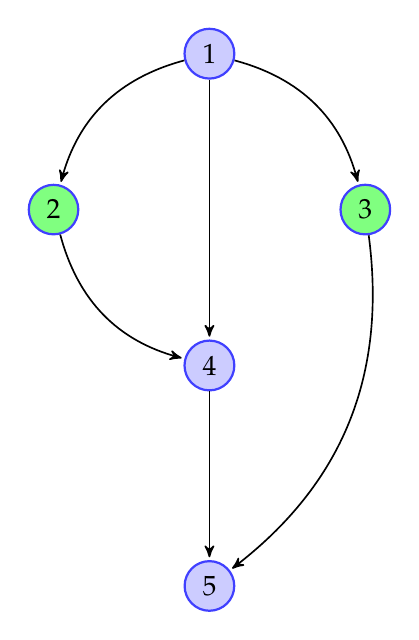
\begin{tikzpicture}[->,>=stealth',shorten >=1pt,auto,node distance=2.8cm,
                    semithick]
    \tikzstyle{place}=[circle,thick,draw=blue!75,fill=blue!20,minimum size=6mm]
  \tikzstyle{red place}=[circle,thick,draw=blue!75,fill=red!75,minimum size=6mm]
  \tikzstyle{green place}=[circle,thick,draw=blue!75,fill=green!50,minimum size=6mm]

  \node[place] (A)                    {1};              
  \node[green place]         (B) [below right of=A] {3};
  \node[green place]         (C) [below left  of=A] {2};
  \node[place]         (D) [below left of=B] {4};
  \node[place]         (E) [below of=D]       {5};



        
  \path (A) edge [bend left]  node {} (B)
            edge [bend right]   node {} (C)
            edge               node{}       (D)
        (C) edge [bend right] node{} (D) 
        (D) edge node{} (E)
        (B) edge [bend left] node{} (E)   
        ;      
\end{tikzpicture}

\caption{Revision diagram of Example 1. In the following diagram the forked revisions are represented by green nodes and the join results by blue. Outgoing arrows represent forks and  joins are represented by incoming arrows, which are always two, one for the joinee and one for the head revision. In the diagram nodes correspond to revisions as follows: 1 - {\tt revision } 2 - {\tt rev1 } 3 - {\tt rev2 } 4 - {\tt join\_rev1 } 5 - {\tt join\_rev2} }
\label{fig1}
\end{figure}
 


\subsubsection{Illegal revision diagrams}
Not all possible joins are legal as some of them might invalidate the assumptions about the flow of revisions.

\begin{figure}[ht!]
\centering


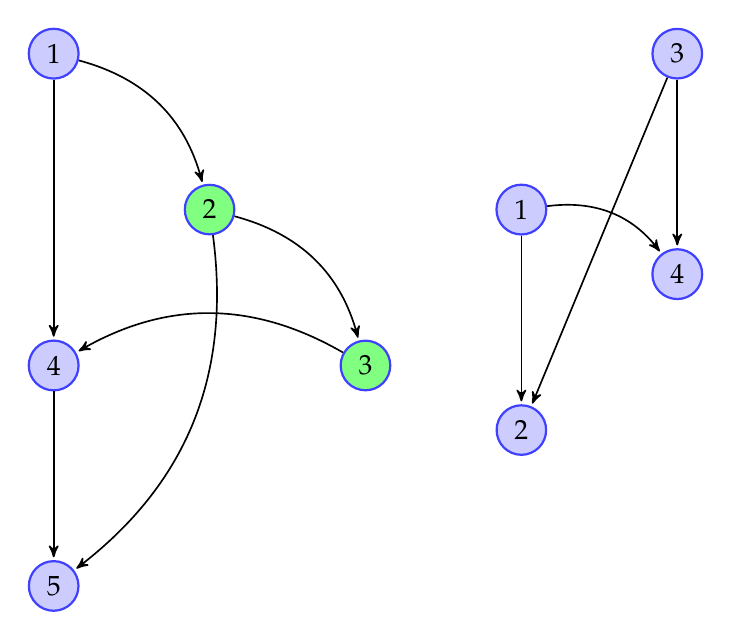
\begin{tikzpicture}[->,>=stealth',shorten >=1pt,auto,node distance=2.8cm,
                    semithick]
    \tikzstyle{place}=[circle,thick,draw=blue!75,fill=blue!20,minimum size=6mm]
  \tikzstyle{red place}=[circle,thick,draw=blue!75,fill=red!75,minimum size=6mm]
  \tikzstyle{green place}=[circle,thick,draw=blue!75,fill=green!50,minimum size=6mm]

  \node[place]         (A)                    {1};              
  \node[green place]         (B) [below right of=A] {2};
  \node[green place]         (C) [below right  of=B] {3};
  \node[place]         (D) [below left of=B] {4};
  \node[place]         (E) [below of=D]       {5};

  \node[place]         (F) [above right of=C]         {1};
  \node[place]        (G) [below of=F]         {2};
  \node[place]         (H) [above right of=F]         {3};
  \node[place]         (I) [below of=H]        {4};
        
  \path (A) edge [bend left]  node {} (B)
            edge               node{}       (D)
        (C) edge [bend right] node{} (D) 
        (D) edge node{} (E)
        (B) edge [bend left] node{} (C)
            edge [bend left] node{} (E)
            
        (F) edge node{} (G)
            edge [bend left] node{} (I)
        (H) edge node{} (I)
            edge  node{} (G)           
        ;      
\end{tikzpicture}
\caption{Illegal revision diagrams.}
\label{fig2}
\end{figure}


In Fig.\ref{fig2} we can see two illegal revision diagrams. In the one on the left, we join revision 3 to revision 1 before we have joined revision 2 which is the parent revision of 3. This means that the result in revision 5 might not be what we would expect since it is unknown how much of the work in the fork for revision 2 was done before forking revision 3. When we join 2, some of the changes occurring (which might have subsequently been modified) in 2 are already joined when 3 was joined. Since the merge function cannot account for such an interleaving as it is chosen by the programmer arbitrarily, such a revision diagram is not valid. One can imagine a more complex concept where this is accounted for at the time of the join. However this would require significantly more programming effort when designing the merge function. This would result in more difficult to reason about concept, prone to programming error. Moreover, this breaks the guarantee that each revision fork is atomic. This would not add extra functionality, since the legal revision diagrams are already expressive enough \cite{conrev}. 

In the example on the right, we are interleaving two separate flows of revisions and there is no way to ensure that they isolate a similar state. This is completely meaningless, since they could isolate different variables and represent unrelated states.





\cleardoublepage



\chapter{Preparation}
\section{The author in the world of concurrency}
As part of my degree I have gained broad knowledge of the problems that arise from concurrency and the typical approaches for solving them. The Concurrent and Distributed Systems course gave me most insight into why and how Concurrent revisions can be used for parallel programming. After reading the original paper, the concept naturally fit in and expanded the mental model I have created about the issues and solutions in the world of Concurrency.  

\section{Familiarizing with the OCaml programming language}
Prior to starting the project, I had almost no experience with the OCaml programming language. For that reason I dedicated the first part of my project to making myself familiar with it. I used the Real World OCaml book \cite{realocaml} to guide me through the concepts and patterns for the language. I was able to quickly transfer and expand my skills in ML into OCaml without much difficulty.

\section{The Core and Async libraries}
I made extensive use of the Core and Async libraries for OCaml. The latter was used in the core of the implementation and the use cases. The {\tt Revision} module (\ref{implementation}) conforms to the pattern of deferred computations in the Async library. This naturally happened in the development process, since the core concepts in the Async library and those of the project complement each other. The revision and isolated data types are completely isolated, making it trivial to implement them as deferred data types and the forks and the joins as deferred computations.  

\section{Back-up and revision control}
For revision control I used git, with which I had a lot of prior experience. I used GitHub for back-up of the code. To insure myself against hardware failure of my personal laptop, I kept my whole development environment inside a VM. The VM was backed up on an external hard drive so in case of system failure I could quickly resume work on another machine.

\cleardoublepage
\chapter{Implementation}
\label{rev_implement}
I have implemented the Concurrent Revisions concept as a library for OCaml. The implementation has passed a series of unit tests and was used for implementing two use cases - a logging and a chat service, as well as a few simple examples.
\section{API}
\label{implementation}
Usage of the library is relatively straight forward and effortless. The user first has to satisfy a module signature called {\tt Isolatable}:

{\scriptsize\noindent\begin{longtable}{r|l}
\mlcodeline{1}{\mlkeywordA{module}~\mlkeyword{type}~Isolatable~\mlkeyword{=}~\mlkeyword{sig}
}
\mlcodeline{2}{~~\mlcomments{(**~Type~{to}~be~isolated~**)}
}
\mlcodeline{3}{~~\mlkeyword{type}~t
}
\mlcodeline{4}{~~\mlcomments{(**~Merge~{function}{\mbox{\COLON}}~merge~{[}head{]}~{[}parent{]}~{[}current{]}~**)}
}
\mlcodeline{5}{~~\mlkeyword{val}~merge\mloperator{\mbox{\COLON}}~t~\mlkeyword{->}~t~\mlkeyword{->}~t~\mlkeyword{->}~t
}
\mlcodeline{6}{\mlkeyword{end}
}
\mlcodeline{7}{
}
\mlcodeline{8}{\mlkeywordA{module}~Make(X\mloperator{\mbox{\COLON}}Isolatable)~\mloperator{\mbox{\COLON}}~
}
\mlcodeline{9}{~(Revision~\mlkeyword{with}~\mlkeyword{type}~value~\mlkeyword{=}~\mlmodulename{X}\mbox{}\mloperator{.}t~\mlkeywordA{and}~\mlkeyword{type}~isolated~\mlkeyword{=}~(int~\mloperator{*}~\mlmodulename{X}\mbox{}\mloperator{.}t)~\mlmodulename{Deferred}\mbox{}\mloperator{.}t)}
\end{longtable}
}

Then from this module, using the {\tt Make} functor, he creates a {\tt Revision} module that satisfies the following signature:
%TC:ignore 
\begin{comment}
module type Revision = sig
  type i
  type result
  type t
  type isolated
  type value

  val init: unit -> t
  (** Adds a new isolated with [value] and returns a new result **)
  val create:  t -> value -> result
  
  (** For breaking the result into revision and isolated **)
  val get_revision: result -> t
  val get_isolated: result -> isolated
  
  (** Scheduling primitives **)
  val fork: t -> (t -> t Deferred.t) -> t Deferred.t
  val join: t -> t -> t
  
  (** Isolated access **)
  val write: t -> isolated -> value -> t
  val read: t -> isolated -> value Deferred.t

  (** Ensures the revision is determined **)
  val determine_revision: t -> t

end
\end{comment}
%TC:endignore 

{\scriptsize\noindent\begin{longtable}{r|l}
\mlcodeline{1}{\mlkeywordA{module}~\mlkeyword{type}~Revision~\mlkeyword{=}~\mlkeyword{sig}
}
\mlcodeline{2}{~~\mlkeyword{type}~i
}
\mlcodeline{3}{~~\mlkeyword{type}~result
}
\mlcodeline{4}{~~\mlkeyword{type}~t
}
\mlcodeline{5}{~~\mlkeyword{type}~isolated
}
\mlcodeline{6}{~~\mlkeyword{type}~value
}
\mlcodeline{7}{
}
\mlcodeline{8}{~~\mlkeyword{val}~init\mloperator{\mbox{\COLON}}~unit~\mlkeyword{->}~t
}
\mlcodeline{9}{~~\mlcomments{(**~Adds~a~{new}~isolated~{with}~{[}value{]}~{and}~returns~a~{new}~result~**)}
}
\mlcodeline{10}{~~\mlkeyword{val}~create\mloperator{\mbox{\COLON}}~~t~\mlkeyword{->}~value~\mlkeyword{->}~result
}
\mlcodeline{11}{~~
}
\mlcodeline{12}{~~\mlcomments{(**~For~breaking~the~result~into~revision~{and}~isolated~**)}
}
\mlcodeline{13}{~~\mlkeyword{val}~get\_{}revision\mloperator{\mbox{\COLON}}~result~\mlkeyword{->}~t
}
\mlcodeline{14}{~~\mlkeyword{val}~get\_{}isolated\mloperator{\mbox{\COLON}}~result~\mlkeyword{->}~isolated
}
\mlcodeline{15}{~~
}
\mlcodeline{16}{~~\mlcomments{(**~Scheduling~primitives~**)}
}
\mlcodeline{17}{~~\mlkeyword{val}~fork\mloperator{\mbox{\COLON}}~t~\mlkeyword{->}~(t~\mlkeyword{->}~t~\mlmodulename{Deferred}\mbox{}\mloperator{.}t)~\mlkeyword{->}~t~\mlmodulename{Deferred}\mbox{}\mloperator{.}t
}
\mlcodeline{18}{~~\mlkeyword{val}~join\mloperator{\mbox{\COLON}}~t~\mlkeyword{->}~t~\mlkeyword{->}~t
}
\mlcodeline{19}{~~
}
\mlcodeline{20}{~~\mlcomments{(**~Isolated~access~**)}
}
\mlcodeline{21}{~~\mlkeyword{val}~write\mloperator{\mbox{\COLON}}~t~\mlkeyword{->}~isolated~\mlkeyword{->}~value~\mlkeyword{->}~t
}
\mlcodeline{22}{~~\mlkeyword{val}~read\mloperator{\mbox{\COLON}}~t~\mlkeyword{->}~isolated~\mlkeyword{->}~value~\mlmodulename{Deferred}\mbox{}\mloperator{.}t
}
\mlcodeline{23}{
}
\mlcodeline{24}{~~\mlcomments{(**~Ensures~the~revision~is~determnined~**)}
}
\mlcodeline{25}{~~\mlkeyword{val}~determine\_{}revision\mloperator{\mbox{\COLON}}~t~\mlkeyword{->}~t
}
\mlcodeline{26}{
}
\mlcodeline{27}{\mlkeyword{end}}
\end{longtable}
}



 
Creation of revisions is performed by the {\tt init} and {\tt create} functions. The former initializes an empty revision and the latter takes a revision and an initial value of the isolated type and returns a {\tt result}. This is a deferred tuple of {\tt Revision.t} and {\tt isolated}. It can then be broken up by the usage of {\tt get\_revision} and {\tt get\_isolated}. This seems a bit awkward to use, but it is enforced by the Async library. Both {\tt Revision.t} and {\tt isolated} are deferred types, however, since {\tt create} is a deferred computation, it has to return a deferred type as well, meaning it cannot return a tuple of deferreds, since in Async each deferred computation has to return a single deferred value.

The scheduling primitives are the trivial {\tt fork} and {\tt join} operations common for asynchronous tasks. Note that they are both purely functional and do not mutate any of the input state and return a fresh revision each time. This makes it explicit whenever the state is changed as this results in creation of a new immutable value. 


Arguments for the operations over revisions are type checked, which significantly reduces the chance of errors on the part of the programmer. Such errors will be reported by the type checker at compile time. When the user implements an illegal revision diagram (see \ref{rev_diag}) the merge often cannot reconcile a valid state, because there is not enough information in the revisions. In that case an exception {\tt Incompatible\_join} is raised. 

There are still some cases when the programmer can implement by error illegal schedules and run them successfully. Ideally these errors should be caught by the type checker, as in the Haskell implementation \cite{haskell}, or by a more elaborate dynamic runtime check, as in the C\# implementation \cite{conrev}.
This is left as a future extension and for now such errors are considered programmer's fault and the behaviour of such is undefined. Undefined behaviour is highly undesirable in a functional environment, especially when doing parallel programming and even more worrying when the aim is to have deterministic behaviour. This issue could potentially be resolved by designing the library as monadic, which is left as a future extension (see \ref{problems} for extended discussion on how this problem could be solved).   

Accessing the isolated variables can be done using the {\tt write} and {\tt read} functions.
Both are also purely functional. The former returns a new revision with the updated value, while the latter returns a deferred value of the regular type which is isolated. In the case when the isolated is not in this revision an exception {\tt Isolated\_Not\_Found} will be raised. Again this is not desirable and can be solved by the extension proposed in the previous paragraph (also see {\ref{problems}). 

The function {\tt determine\_revision} is used to ensure that a revision is evaluated and not merely scheduled for evaluation. Initially the library was not intended to provide such functionality, however during the design of the use cases the need became apparent and I added it to the implementation.


\section{Revisions behind the curtains - data structures}
The internal structure of the revisions is implemented by the following data type:

{\scriptsize\noindent\begin{longtable}{r|l}
\mlcodeline{1}{\mlkeyword{type}~t~\mlkeyword{=}~\mloperator{\{}~parent~\mloperator{\mbox{\COLON}}~((int\mloperator{\mbox{,}}~\mlmodulename{Isolated}\mbox{}\mloperator{.}t\mloperator{\mbox{,}}~\mlmodulename{Int}\mbox{}\mloperator{.}comparator\_{}witness)~\mlmodulename{Map}\mbox{}\mloperator{.}t)\mloperator{\mbox{\SC}}
} 
\mlcodeline{2}{~~~~~~~~~~~self~\mloperator{\mbox{\COLON}}~((int\mloperator{\mbox{,}}~\mlmodulename{Isolated}\mbox{}\mloperator{.}t\mloperator{\mbox{,}}~\mlmodulename{Int}\mbox{}\mloperator{.}comparator\_{}witness)~\mlmodulename{Map}\mbox{}\mloperator{.}t)\mloperator{\mbox{\SC}}
}
\mlcodeline{3}{~~~~~~~~~~~written~\mloperator{\mbox{\COLON}}~\mlmodulename{WrittenSet}\mbox{}\mloperator{.}t\mloperator{\mbox{\SC}}
}
\mlcodeline{4}{~~~~~~~~~~~id~\mloperator{\mbox{\COLON}}~int~
}
\mlcodeline{5}{~~~~~~~~~\mloperator{\}}~\mlmodulename{Deferred}\mbox{}\mloperator{.}t}
\end{longtable}
}

It is a deferred record type which contains two maps that map isolated variables to their value in the parent or the current revision respectively. There is also a written set that keeps track of which isolated variables have been updated in order to improve the performance at join time. In that way, {\tt join} has to deal only with the isolated variables that have been modified. The {\tt Isolated.t} is itself implemented simply as an integer value that is used as a key into the maps. The {\tt id} field in the revision type keeps track of the id of the last created isolated in that revision chain to ensure uniqueness of ids. 

The reasons for choosing these particular data structures are explained in section \ref{design_decisions}.  

\section{Bank transactional example}

Here is the actual implementation of the pseudo-code in Example 1 (\ref{example}):
\label{rev_in_ocaml}

%TC:ignore 
\begin{comment}One of its advantages over the C\# implementation is that it is purely functional and the type checker catches some of the typical mistakes that can be made - trying to access an isolated of a wrong type or join revisions of different types. What it does not do however is check for all types of illegal revision diagrams, instead an exception is raised whenever an illegal join is executed. This is far from ideal and statically type-checking joins for compatibility could be implemented as a future extension (see \ref{problems}).

The API that the implementation exposes to the user is intuitive and resembles the typical OCaml approach for APIs for external libraries. Here is a simple example of its usage:
\end{comment}
\begin{comment}
module IntRevision = Make(struct
    type t = int
    let merge head parent current = head + current - parent
  end)

let () =
  let r = IntRevision.init () in
  let res1 = IntRevision.create r 0 in
  let revision = IntRevision.get_revision res1 
   and account = IntRevision.get_isolated res1 in
     Deferred.both 
      (IntRevision.fork revision 
        (fun r -> 
          return (IntRevision.write r account 
                    ((IntRevision.read r account) + 5)))
      (IntRevision.fork revision 
        (fun r -> 
          return (IntRevision.write r account 
                    ((IntRevision.read r account) + 10)))
     >>|(fun (rev1, rev2 ->
        let join_rev1 = IntRevision.join revision rev1 in
        let join_rev2 = Intrevision.join join_rev1 rev2 in
          assert(IntRevision.read join_rev2 = 15)    
\end{comment}
%TC:endignore 

{\scriptsize\noindent\begin{longtable}{r|l}
\mlcodeline{1}{\mlkeywordA{module}~IntRevision~\mlkeyword{=}~Make(\mlkeyword{struct}
}
\mlcodeline{2}{~~~~\mlkeyword{type}~t~\mlkeyword{=}~int
}
\mlcodeline{3}{~~~~\mlkeywordA{let}~merge~head~parent~current~\mlkeyword{=}~head~\mloperator{+}~current~\mloperator{-}~parent
}
\mlcodeline{4}{~~\mlkeyword{end})
}
\mlcodeline{5}{
}
\mlcodeline{6}{\mlkeywordA{let}~()~\mlkeyword{=}
}
\mlcodeline{7}{~~\mlkeywordA{let}~r~\mlkeyword{=}~\mlmodulename{IntRevision}\mbox{}\mloperator{.}init~()~\mlkeywordA{in}
}
\mlcodeline{8}{~~\mlkeywordA{let}~res1~\mlkeyword{=}~\mlmodulename{IntRevision}\mbox{}\mloperator{.}create~r~0~\mlkeywordA{in}
}
\mlcodeline{9}{~~\mlkeywordA{let}~revision~\mlkeyword{=}~\mlmodulename{IntRevision}\mbox{}\mloperator{.}get\_{}revision~res1~
}
\mlcodeline{10}{~~~\mlkeywordA{and}~account~\mlkeyword{=}~\mlmodulename{IntRevision}\mbox{}\mloperator{.}get\_{}isolated~res1~\mlkeywordA{in}
}
\mlcodeline{11}{~~~~~\mlmodulename{Deferred}\mbox{}\mloperator{.}both~
}
\mlcodeline{12}{~~~~~~(\mlmodulename{IntRevision}\mbox{}\mloperator{.}fork~revision~
}
\mlcodeline{13}{~~~~~~~~(\mlkeyword{fun}~r~\mlkeyword{->}~
}
\mlcodeline{14}{~~~~~~~~~~return~(\mlmodulename{IntRevision}\mbox{}\mloperator{.}write~r~account~
}
\mlcodeline{15}{~~~~~~~~~~~~~~~~~~~~((\mlmodulename{IntRevision}\mbox{}\mloperator{.}read~r~account)~\mloperator{+}~5)))
}
\mlcodeline{16}{~~~~~~(\mlmodulename{IntRevision}\mbox{}\mloperator{.}fork~revision~
}
\mlcodeline{17}{~~~~~~~~(\mlkeyword{fun}~r~\mlkeyword{->}~
}
\mlcodeline{18}{~~~~~~~~~~return~(\mlmodulename{IntRevision}\mbox{}\mloperator{.}write~r~account~
}
\mlcodeline{19}{~~~~~~~~~~~~~~~~~~~~((\mlmodulename{IntRevision}\mbox{}\mloperator{.}read~r~account)~\mloperator{+}~10)))
}
\mlcodeline{20}{~~~~~\mloperator{>\mbox{}>\mbox{}|}(\mlkeyword{fun}~(rev1\mloperator{\mbox{,}}~rev2~\mlkeyword{->}
}
\mlcodeline{21}{~~~~~~~~\mlkeywordA{let}~join\_{}rev1~\mlkeyword{=}~\mlmodulename{IntRevision}\mbox{}\mloperator{.}join~revision~rev1~\mlkeywordA{in}
}
\mlcodeline{22}{~~~~~~~~\mlkeywordA{let}~join\_{}rev2~\mlkeyword{=}~\mlmodulename{Intrevision}\mbox{}\mloperator{.}join~join\_{}rev1~rev2~\mlkeywordA{in}
}
\mlcodeline{23}{~~~~~~~~~~\mlkeyword{assert}(\mlmodulename{IntRevision}\mbox{}\mloperator{.}read~join\_{}rev2~\mlkeyword{=}~15)~~}
\end{longtable}
}


Example 2.\\

From line 1 to 4 we create the {\tt IntRevision} module using a simple anonymous module specifying the type of the isolated data and the merge function. Then on line 7 we initialize an empty revision and on 8 we add a new isolated to the initial revision to create a new one. We then fork the two asynchronous account credits (line 11 to 19) and later join them. 

%TC:ignore 
\begin{comment}
This API is not as straight forward as the one in the C\# implementations for couple of reasons, which makes the usage of revisions a bit more verbose and tedious, but has the benefit of clarity of the programming logic. Since the implementation is purely functional, revisions are immutable which requires to create a new revision at each join. We also need to explicitly create new isolated variables. For evaluation of the API see \ref{eval_api} 
\end{comment}
%TC:endignore 
\section{Design decisions}
\label{design_decisions}
The key aims of the design were to produce a solution that is purely functional, as well as efficient. The desire for a purely functional approach was driven by the necessity of tracking effects of concurrent executions. Purely functional implementation ensures that no side effects occur to the isolated variables inside the revisions. Ideologically changes happen only when revisions are joined. The benefit of this is that modifications of the state are explicit and easy to track both for the programmer and the run time. 

Another advantage of this design decision, comes from the fact that in OCaml complex data structures which are immutable, such as maps, allocate more memory only when the structure is changed. They reuse as much as possible of the internals of the initial structure (chapter \ref{datastruct_core}). This makes replication very cheap both in terms of time and space.

The main design choice for the implementation was how to implement the revisions internally. The obvious choice for the mapping of isolated variables to values was between hash tables and maps. The former would have given constant time for all the update and add operations \cite{cormen}. However, in OCaml hash tables are usually implemented as mutable data structures. Their imperative nature would have broken the functional model of operation for the library. I could have hidden under the curtains the fact that I am using a mutable data structure by lazy replication. This would mean that upon creating a new revision, the structure representing the parent of this revision (which would be a hash table) would have to be replicated explicitly and values would be added to the current revisions only after writes. This would increase the time and space complexity of forks and joins linearly in terms of the number of isolated variables since each of these operations would have to explicitly replicate the whole hash table containing all isolated values. 

The functional nature that I was aiming for required creating a new revision after each operation (either fork, join or addition of a new isolated variable). This makes the creation of new revisions the most common action by the library and shifting from constant to linear complexity was highly undesirable. Taking this consideration into account I made the choice of using maps in the internal structure of the revisions. I used the implementation of maps in the Core library. As mentioned in section \ref{datastruct_core}, they are implemented as self-balanced binary search trees, which provide logarithmic complexity for all reads and writes to their structure. Since only insertion and update operations were performed on the maps, all operations on maps we use are of logarithmic time. What is more, since maps in OCaml are purely functional, they reuse a lot of their internal structure and there is no duplication of data. 

\section{Complexity}
\label{complexity}
Forking a new revision does not require additional space as the revision structure of the parent is not changed and the forked revision merely points to it. The functional nature of the implementation guarantees that the parent would never be mutated, making this way of replication completely safe. Inside the fork, the only operation that requires extra space is {\tt Revision.write}. It has to change the value of an isolated in a revision. Under the hood this is implemented as a value update in a map. This takes just O(log n) time, where n is the number of isolated in that revision and just constant space due to the immutable nature of Core maps and the re-usage of their internal structure. 

In similar fashion to forks, joins also create a new revision, heavily reusing the map from the revision to which we are joining. For every variable changed in the joinee, three values have to be read - from the head revision, the parent revision and the current revision. This takes logarithmic time in terms of the number of isolated variables. Then for each written variable, the merge function is called and the result of it is applied to the head revision, creating a new one. This takes time O(k*log n*merge), where merge is the runtime complexity of the merge function, k is the number of variables changed in the joinee and n is the total number of variables in the revision. The join performs k updates to values in the map, which means it has space complexity of O(k + merge), where merge is the space complexity of the merge function. 

Everything allocated in the merge function is garbage collected after it is executed, which means it does not add extra space complexity to the total runtime. Revisions created by the forks and join would also be garbage collected once they are out of scope, which means space usually is used only for forks not yet joined and the head revisions. We will see how this works in practice with the use cases later on (see \ref{logging} and \ref{chat_server}). 

In total, a sequence of k forks and joins, n isolated variables, r reads and w writes gives a total runtime overhead of using revisions of O(r*log n + w*log n + k + w*log n) = O((r+w)log n). In most use cases n is a small number, which means that we could regard log n as a constant. This results in unaffected time complexity of the initial algorithm the user is implementing. For example the use cases of a logging and a chat system, discussed in chapters \ref{logging} and \ref{chat_server}, use only a single isolated. Even when a large number of isolated is needed, we still get only logarithmic overhead. However, using an alternative approach to concurrency would need a more elaborate synchronization scheme that would rely on blocking or roll-backs which in a concurrent system would waste a lot of CPU time or cause delays when conflicts arise. This would typically be much greater than the overhead of revisions. What is more, alternative approaches require significantly more effort from the programmer.

In terms of space, the runtime of revisions adds just a constant overhead for each write, which does not affect the space complexity of the algorithm.     

    

\section{Error handling}
\label{errors}
There are two classes of runtime errors that the implementation has to deal with.
 
The first one is concerned with illegal usage of revisions. When a read or write of an isolated from a revision is executed, there is still no guarantee that the revision contains a value for this particular isolated, even when their compatibility was successfully type-checked. In that case an exception {\tt Isolated\_Not\_Found} is raised. When the run-time discovers an illegal join (note that not all of these are caught, see {\ref{problems}), it raises an {\tt Incompatible\_join} exception.

The second class of runtime errors are those occurring in the user declared code to be executed inside the revisions framework - namely the merge function and the functions executed inside forks. For the former the exceptions are left uncaught, since merely abandoning joins would result in a silent failure, which would be difficult to debug. As for the latter - the exception is caught inside the fork and only re-raised if the fork is joined. Since results of forks are only applied to the state after the join it is consistent with the concept to treat exceptions as any other state changes.  
 
\section{Unit tests \& example code}
 A number of unit test were designed which cover all possible legal revision diagrams and a different number of isolated variables. They were used in parallel with the ongoing work on the implementation to ensure its correctness. 
 
 The simple examples from the original paper were also implemented. These include the previously discussed example of isolating integers (see \ref{rev_in_ocaml}), a "Hello World" example using isolated strings and an example demonstrating the benefits of re-raising fork exceptions when revisions are joined, which provides efficient tools for roll-backs of revisions.
  
\section{Use case - Logging system}
\label{logging} 
The first use case I designed using the library was a distributed logging service. In this use case there is one central server that receives log messages from multiple clients and merges them into a single log stream. 

\subsection{Motivation}
Performance of distributed systems could typically be improved by using extra concurrency. One such example is this type of logging system. 
As this is a distributed system with centralized service, responsiveness and scalability is required at the server end, which is the bottleneck of the whole system. The former could be achieved by adding extra concurrency and the latter by exploring hardware parallelism. However, naively applying concurrency in such a system would introduce a lot of non-determinism. Distributed message passing between clients and the server could suffer from random delays and message processing can be reordered by the runtime behaviour of the server. The service that this system should provide should be deterministic and log messages should be totally ordered.

This is an excellent field to use Concurrent revisions to introduce concurrency in a deterministic way and increase responsiveness. My implementation of revisions do not explore hardware parallelism due to the OCaml runtime limitation for this. However, by reducing the synchronization logic at the server side, the implementation could become more scalable as synchronization becomes less expensive and processing messages could be done more efficiently.

\subsection{Features}
The system provides only three features:
\begin{itemize}
\item
Registration of new logging clients
\item
Logging messages from the clients
\item
Dumping the log history to a local file at the server side upon request from a client
\end{itemize}

Although this system does not provide a lot of features, what complicated its design were the required guarantees:
\begin{itemize}
\item
Messages from a single clients should not be reordered in the global log stream
\item
Logged messages should never be lost
\item
Messages from different clients should be ordered in the stream by their locally taken timestamps
\end{itemize}

This requires care to be taken when merging a new message to the stream. More importantly - the clearly defined total order on log messages (modulo clash of timestamps up to milliseconds) suggests a deterministic run-time behaviour.

For the purpose of this project I am using locally taken timestamps in the clients to impose that order. The alternative would be order by the absolute logging time of messages, which would require distributed message passing ordering, which is beyond the scope of this project and does not relate to its purpose \cite{bacon}. 

\subsection{Implementation}
\label{log_imp}
I will focus on the implementation of the server as it the bottleneck of the system and could benefit significantly more from increased concurrency.

\subsubsection{State representation}
The state of the system is represented by a module {\tt RepMessage} that wraps around a map from timestamps to messages and provides the basic functionality required over the stream of log messages (for an extended discussion of the functionality of the module see \ref{ser_rep}). 

\subsubsection{Usage of Concurrent revisions}
\label{log_usage}
The state that has to be isolated and consistently updates is the stream of log messages itself. I declared {\tt RepMessage.t} (see \ref{ser_rep}) as the type to be isolated. Then I created a revision module using the library I implemented for Concurrent revisions for operating over this isolated state. 

My initial aim was for a purely functional design, this however turned out to limit concurrency significantly and would impose completely sequential order on events (see section \ref{eval_imp} for the reasoning behind this}). One way to work around this issue would to be use monadic design which would allow tracking of state changes \cite{monad}. However, this seems a bit of an overkill for this simple use case. Instead I decided to use a global reference to the head revision, which is read by each fork and written by each join.

After arming myself with a Concurrent revision module that allows forking and joining asynchronous tasks that mutate the global state, there was one more concern - how to resolve conflicts. In the concept of revisions there is an explicit place where to do that - the merge function. This function has to deterministically add new messages to the stream, keeping them in order and ensuring no messages are lost. Conflicts can only arise from messages added to the stream so only this case has to be dealt with by the merge function. This function takes three arguments - the current state, the state at the time of the fork and the state containing the changes made inside the fork. For optimization purposes the last processed message is also kept with the state, otherwise the merge function would have to take the union of two stream which would be expensive. What it does instead is looking at this last message timestamp and add it to the appropriate place in the current state. Since the use case is fairly simple, the merge function do not examine the streams in its last two arguments.

\subsubsection{Runtime flow}
Each user that wants to communicate with the server opens a TCP connection with it. Then the server and the clients exchange commands that are predefined and are shared between them as communication protocol. They are passed around serialized as s-expressions. S-expressions are an efficient serialization technique in OCaml, based on well bracketed expressions. A simple example of s-expression would be {\tt (this (is an) (s expression))}. 

The design of the server is based on a two-stage producer-consumer solution. The clients produce events, which are consumed by asynchronous concurrent forked revisions. Once evaluated these revisions are consumed by a second stage which joins them to the global state. 

All the connections are served in parallel and messages are added to a pipe as they arrive without blocking. A recursive function takes messages out of this pipe and forks a new revision corresponding to each message. The forked revisions are just scheduled for evaluation without blocking the function that takes messages out of the pipe, which means that at any given time there can be arbitrary many fully parallelized forks. 

Again in full parallel, the revisions of that result from the forks are added to another pipe after they have been determined. Another recursive function takes revisions (which are already determined) and joins them one by one to the global state. Note that this function will never block waiting for a revision coming from the pipe to be determined as all revisions in the pipe are guaranteed to already have been evaluated. Parallelizing the joins is not possible as this will result in invalid revision diagram, which diverges indefinitely without even converging to a globally consistent state. Having said that, the run-time of the server is as concurrent as the concurrent revisions concept allows for (see \ref{eval_join} for discussion on this).

Updating a reference at the end of the join, which is also dereferenced at the forking time and in the beginning of the join, is safe since all deferred computations in Async are atomic and guarantee that consistent global state is always seen both by the forks and the joins. 

The revision digram of the run-time of the server is shown in Fig.\ref{fig3}

\begin{figure}[ht!]
\centering


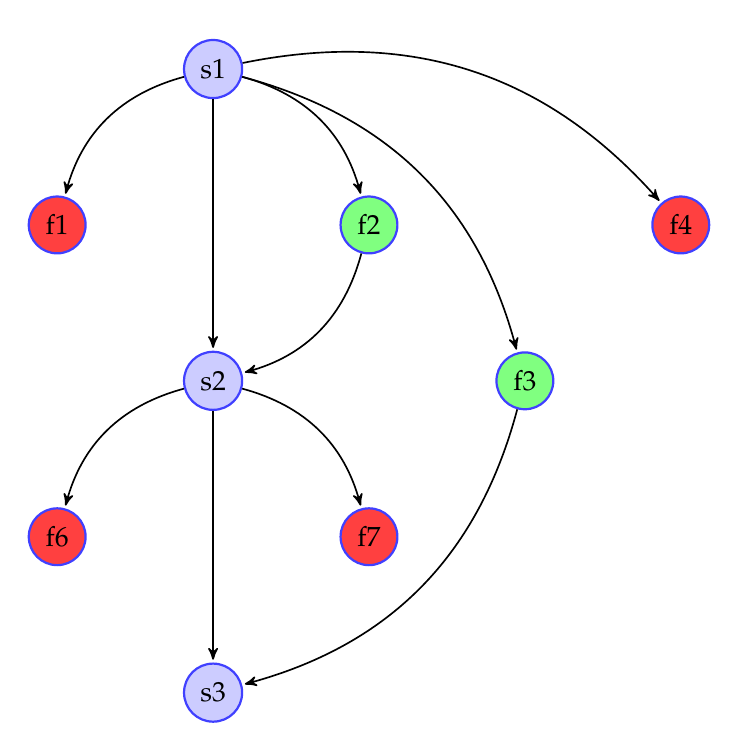
\begin{tikzpicture}[->,>=stealth',shorten >=1pt,auto,node distance=2.8cm,
                    semithick]
  \tikzstyle{place}=[circle,thick,draw=blue!75,fill=blue!20,minimum size=6mm]
  \tikzstyle{red place}=[circle,thick,draw=blue!75,fill=red!75,minimum size=6mm]
  \tikzstyle{green place}=[circle,thick,draw=blue!75,fill=green!50,minimum size=6mm]

  \node[place] (A)                    {s1}; 
  \node[red place] (B) [below left of=A] {f1};
  \node[green place] (C) [below right of=A] {f2};
  \node[green place] (D) [below right of=C] {f3}; 
  \node[red place] (E) [above right of=D] {f4}; 
  \node[place] (F) [below right of=B] {s2};
  \node[red place] (G) [below left of=F] {f6};
  \node[red place] (H) [below right of=F] {f7};             
  \node[place] (I) [below right of=G] {s3}; 
  
  \path (A) edge [bend left]  node {} (C)
            edge [bend right] node {} (B)
            edge [bend left]  node {} (D)
            edge [bend left]  node {} (E) 
            edge []             node {} (F) 
        (C) edge [bend left]  node {} (F) 
        (F) edge [bend left]  node {} (H)
            edge [bend right] node {} (G)
            edge []           node {} (I) 
        (D) edge [bend left] node {} (I);
  
   
\end{tikzpicture}
\caption{Revision diagram of example flow in the logging server. Here the blue nodes denote revisions keeping the global state, red nodes - not joined yet fork revisions and green nodes - joined fork revisions. It this example from state s1 are forked four revisions (the number of forked revisions is not constrained, it depends only on task interleaving). When revision f2 is joined to the state, the global state is updated to the result of the join - s2. Any fork that is joined afterward is joined to this new state (unless it has been updated again of course), an example of which is f3, which was forked by s1, but joined to s3. }
\label{fig3}
\end{figure}

\section{Use case - Chat server}
\label{chat_server}
\subsection{Motivation}

Much like the logging system, a chat system is highly distributed, has a lot of conflicts that have to be resolved deterministically and requires scalability and limited delays. Such a system can benefit significantly from concurrency, which could allow for more clients to be served and to limit the delays that these clients might experience.

This is clearly a trivial problem, implemented numerous times before. Examples of widely successful distributed chat systems are WhatsApp, Facebook chat, Skype. However, it is interesting to see what could be achieved if implemented using Concurrent revisions. I am focusing on a less general case which centralizes the system around a single server providing services to multiple clients. I choose this use case since it is exemplary for a problem where we need a lot of concurrency, but without sacrificing consistency. 

The aim of the chat system implementation is not to be optimized for the particular problem of exchanging personal messages, but rather to be a witness for an arbitrary parallel system. Applying revisions to it and measuring performance between a version with revisions and one less parallel without revisions could give valuable insight on the usability of my library, the performance improvement and the overhead of using revisions. Since the user interface of the client has no connection to the performance inside the server and the qualities I was trying to examine, I paid a little attention to it.   

The core component of interest is the chat server itself, since it is the one that has to provide adequate and fair service to all the clients and the only way to achieve this is to add concurrency while keeping consistent state.

\subsection{Features}
The following features were implemented for both versions of the server:
\begin{itemize}
\item
Registration of new users
\item
Creating, joining and leaving chat rooms
\item 
Sending messages to chat rooms
\item
Promoting users to admin status in a particular room
\item
Merging chat rooms
\end{itemize}
  
\subsection{Implementation using Concurrent revisions}
\label{chat_par}

Much like the logging system, the chat server has to keep a reference to the head revision as a global mutable state in order to serve all users consistently (see \ref{log_usage} for clarification and \ref{eval_imp} for reasoning behind this). 

\subsubsection{Data types}
\label{ser_rep}
The state of the server is of type:

%TC:ignore 
\begin{comment}
type st = 
  { id:int; 
    rooms: RepRoom.t; 
    users: RepUser.t; 
    last_event: command; 
    last_event_time: Time.t
  } 
\end{comment}
%TC:endignore 

{\scriptsize\noindent\begin{longtable}{r|l}
\mlcodeline{1}{\mlkeyword{type}~st~\mlkeyword{=}~
}
\mlcodeline{2}{~~\mloperator{\{}~id\mloperator{\mbox{\COLON}}int\mloperator{\mbox{\SC}}~
}
\mlcodeline{3}{~~~~rooms\mloperator{\mbox{\COLON}}~\mlmodulename{RepRoom}\mbox{}\mloperator{.}t\mloperator{\mbox{\SC}}~
}
\mlcodeline{4}{~~~~users\mloperator{\mbox{\COLON}}~\mlmodulename{RepUser}\mbox{}\mloperator{.}t\mloperator{\mbox{\SC}}~
}
\mlcodeline{5}{~~~~last\_{}event\mloperator{\mbox{\COLON}}~command\mloperator{\mbox{\SC}}~
}
\mlcodeline{6}{~~~~last\_{}event\_{}time\mloperator{\mbox{\COLON}}~\mlmodulename{Time}\mbox{}\mloperator{.}t
}
\mlcodeline{7}{~~\mloperator{\}}~}
\end{longtable}

}

The state keeps track of the last event and its timestamp for synchronization purposes, which I will later explain along with the merge function invoked when joining revisions in the next subchapter.

The two modules {\tt RepRoom} and {\tt RepUser} encapsulate the representation of the ordered set of rooms and users respectively in the state of the server. Under the hood the types {\tt RepRoom.t} and {\tt RepUser.t} are implemented as maps with keys the ids of the users and the rooms and data type {\tt chat\_room} and {\tt user}. These types have the following signatures:
%TC:ignore 
\begin{comment}

type user =
  { id : int;  
    su : bool;
    name : string;
    reader : Reader.t;
    writer : Writer.t;
  }

type chat_room = 
  { history : RepMessage.t;
    users : RepUser.t;
    id : int;
  }
  
\end{comment} 
%TC:endignore   
{\scriptsize\noindent\begin{longtable}{r|l}
\mlcodeline{1}{\mlkeyword{type}~user~\mlkeyword{=}
}
\mlcodeline{2}{~~\mloperator{\{}~id~\mloperator{\mbox{\COLON}}~int\mloperator{\mbox{\SC}}~~
}
\mlcodeline{3}{~~~~su~\mloperator{\mbox{\COLON}}~bool\mloperator{\mbox{\SC}}
}
\mlcodeline{4}{~~~~name~\mloperator{\mbox{\COLON}}~string\mloperator{\mbox{\SC}}
}
\mlcodeline{5}{~~~~reader~\mloperator{\mbox{\COLON}}~\mlmodulename{Reader}\mbox{}\mloperator{.}t\mloperator{\mbox{\SC}}
}
\mlcodeline{6}{~~~~writer~\mloperator{\mbox{\COLON}}~\mlmodulename{Writer}\mbox{}\mloperator{.}t\mloperator{\mbox{\SC}}
}
\mlcodeline{7}{~~\mloperator{\}}
}
\mlcodeline{8}{
}
\mlcodeline{9}{\mlkeyword{type}~chat\_{}room~\mlkeyword{=}~
}
\mlcodeline{10}{~~\mloperator{\{}~history~\mloperator{\mbox{\COLON}}~\mlmodulename{RepMessage}\mbox{}\mloperator{.}t\mloperator{\mbox{\SC}}
}
\mlcodeline{11}{~~~~users~\mloperator{\mbox{\COLON}}~\mlmodulename{RepUser}\mbox{}\mloperator{.}t\mloperator{\mbox{\SC}}
}
\mlcodeline{12}{~~~~id~\mloperator{\mbox{\COLON}}~int\mloperator{\mbox{\SC}}
}
\mlcodeline{13}{~~\mloperator{\}}}
\end{longtable}
}

The record type {\tt user} has {\tt id} and {\tt name} fields for the id and name of the user respectively. A user is also specified by whether he has admin privileges - {\tt su}, and {\tt writer} and {\tt reader} fields that are descriptors used by the {\tt Readed} and {\tt Writer} modules in Async. They are used for reading from and writing to the TCP connection to each client in an even-driven manner.

The chat rooms also have ids, along with an a list of users (provided by the {\tt RepUser} module) and chat history provided by the {\tt RepMessage} module.

The modules {\tt RepMessage}, {\tt RepUser} and {\tt RepRoom} are used for refactoring the implementation of the server. They all have type {\tt t} implemented as a map that maps ids (for users and rooms) and timestamps (for messages) to the types representing messages, users and rooms respectively. These modules provide the basic functions required for dealing with ordered sets of these types. Because of the implementation of maps in the Core library, discussed in \ref{datastruct_core}, all the updates done by these modules take logarithmic time and constant space.     

\subsubsection{Usage of Concurrent Revisions}

As mentioned in the beginning of the previous subsection, the inherited nature of the chat server requires a global mutable state. I implemented this as a reference to a revision with isolation type {\tt st} (discussed above). There is only a single isolated that is the state of the server in the particular revision. This means that reads and writes of isolated take only constant time and space for reasons explained in chapter \ref{complexity}.

Unpredictable network delays could reorder events reaching the server. This could be overcome by introducing a partial order to the distributed message passing \cite{bacon}, which however adds significant complexity and is also out of the scope of this project. For the purpose of this implementation, I consider only determinism based on event timestamps, taken when the events are received at the server.

The most interesting part of the usage of revisions is the merge function. It operates on the current consistent state of the server and the state that has come from the fork. Keeping the timestamp of the last event in the state allows the merge function to account for some delayed processing of events. That way it can deal with conflicts which have to be resolved by incorporating effects of events according to their initial timing. Access to the last event from the state is done merely as an optimization, otherwise the merge would have to scan the whole state to find changes instead of only the areas that could have been changed. The reason for this is one of the limitations of the implementation of the library - ideally we would like the user list and each room to be isolated separately, however my implementation do not allow a revision to have isolated of different types, for reasons explained in chapter \ref{rev_in_ocaml}. Given that it was not too difficult to deal with that limitation I do not consider it a major issue. 

The merge function also has to account for many possible sequences of events that could introduce conflict which have to be resolved deterministically in order to keep the deterministic change of the state. Let's take a look at some of these special cases.

Consider the case when two users simultaneously try to register with the server with the same name. A new revision is forked for each of the registration events. The function evaluated in the fork has a consistent snapshot of the state at the time of the fork, but is not aware of what is happening in the other fork, since they are asynchronous. Given the name the users try to register with is not already in use, both forks will succeed resulting in two new revisions ready to be joined to the global state. This introduces a conflict - having two users with the same name in the two revisions we have to join. 

This is where the merge function I supplied when isolating the state shines. When joining the first revision everything works fine and the result of the join is assigned to the global state. When joining the other revisions however, it is joined to the new global state which already has the first user registered. The merge function can now look at the list of users in the head revision and find out the user name is already in use. Then it can abort the join and inform the client for the fail without introducing inconsistency in the state of the server. Unfortunately there is still a bit of non-determinism - the user that succeeds is not necessary the one that tried to register first. Alternatively the merge function could take into account the timestamp of each registration event and ensuring the first user is the one registered. This would mean that the second user could potentially be registered and later on thrown out of the server, which is an undesirable poor user experience. The same reordering can happen because of network delays as well. Implications of this are discussed in chapter \ref{eval_nondet}.

Another example of a special case is when a new user enters a chat room and another user sends a message to the same room after that, the effect of the second event is joined first to the state. The merge function can easily deal with that as well - it can simply compare the timestamp of the registration with the timestamps of the messages in the room history and send the last message to the newly registered user.

The final example I would like to point out is the special case of merging two chat rooms. This means that that messages from both groups have to be put in the right order and the union of lists of users has to be taken. This can trivially be done inside the fork, since both the history and the user lists are implemented as maps. However, before the result of that is joined to the head revisions, some other users and messages could have been added to one of the rooms. The merge function once again deals with that by checking the timestamp of the merge event to make sure all new messages are added accordingly and checks once again that a user is in the resulting user list if and only if it is in one of the groups at the head revision.

\subsubsection{Runtime flow}

The runtime flow for the chat server is almost identical to that in the logging server (\ref{log_imp}). However, here the merge function deals with more different flavours of conflicts. Not all of them can be resolved - example of which is two users trying to register with the same name simultaneously. In that case the conflict has to be resolved in collaboration with the client. When such a conflict occurs, the merge function simply discards the failed revision and inform the unlucky user for the name conflict. 

Apart from that the runtime flow is exactly the same as in Fig.\ref{fig3}

\subsection{Implementation without Concurrent revisions}
\label{imp_no}
I implemented a second version of the chat server which does not make use of Concurrent revisions. The functionality and state representation is exactly the same as for the other version, discussed in \ref{ser_rep}. 

What is different is the runtime flow. In this version events from clients are still accepted concurrently, but they are processed in a sequential manner. This significantly reduces concurrency inside the implementation. 

It should also be noted that the concurrent version has to perform about three times more work per a command compared to the sequential version. The former has to check if a fork is required, perform the computation inside the fork and then merge the fork resolving any conflicts. The sequential version merely has to perform what is effectively the second stage of what happens in the other version.

The performance of both versions of the chat server is discussed in \ref{perf_eval}.


\cleardoublepage
\chapter{Evaluation}

\section{Usability evaluation}
The implementation of the use cases (see \ref{logging} and \ref{chat_server}) showed that from development perspective, using the implementation of the library provided the necessary functionality to achieve the desired goals and did not require major workarounds and head-scratching how to bend the rules to get the desired outcome. There were however a few design choices imposed by the library that require careful evaluation. There are also some concerns about the guarantees that the library provides. Both of these are discussed bellow.

\subsection{Evaluation of the API for the use cases}
\label{eval_api}
As stated in chapter \ref{rev_in_ocaml}, the API of my library is somehow more verbose and heavy to use. In the C\# implementation the user simply declares which variables have to be isolated and then uses them as any regular variables. The solution in the project implementation is a bit less convenient - it uses special read and write methods, to which the context has to be explicitly stated. However, it makes it much clearer what is actually isolated, when it is accessed and in what context, resulting in a more comprehensive logic.  

Another drawback of my implementation is that it does not allow having isolated from different types in a single revision, a trivial workaround for which is to use tuples or another complex data structure. 

In the chat server implementation we saw that joining revisions could be more natural and efficient if the different components of the state could be isolated separately allowing for a more fine grained merge functions (see \ref{chat_par}-Implementation using Concurrent revisions}). In this case the workaround of using a complex data type increases the demand from the programmer. Isolating a variant type, however, could allow the user to effectively isolate a predefined set of different types and specify a single merge function that processes the distinct branches of the variant type separately allowing for such a fine grained control. This limitation of the library turns out to cripple neither the performance nor the usability, it merely requires an alternative approach from the programmer.  

\subsection{Need for imperative structure for the use cases}
\label{eval_imp}
In the implementation of the use cases (sections \ref{logging} and \ref{chat_server}) I needed to resort to a less satisfying to my taste not purely functional implementation. At first glance this looked like a limitation of the concept.

For the logging service and the chat server the reason for this is that each processing of a new event that would change the state and the merging of its effects has to operate on a consistent state of the server and once the state is changed successfully, new events have to be processed according to the new state. Achieving this in a purely functional manner will require passing the state as an input argument to the function serving the requests. If this function is recursive then this input parameter could be used as a running state. However, this does not provide any concurrency at all since the same running state should be updated by the merge function.

This inherited flow of state changes in the use cases show that the need of a global mutable state is not a limitation of the concept or the implementation. Rather, it is imposed by the problem which the use cases try to solve itself.  

\subsection{Possibility of non-determinism introduction}
\label{eval_nondet}
The merge function for conflict resolution is declared by the programmer himself. There are no restrictions imposed by the library on this function, apart of its type. This means that the programmer could introduce non-determinism in the whole flow of revisions by the door left in the merge function. One could argue that this leaves room for errors due to unintentional creeping in of non-determinism when it is not desirable. This is indeed true, however, disallowing the possibility of non-pure behaviour in the merge function could limit the usability for the cases where the problem requires non-deterministic conflict resolution.
  
In section \ref{log_imp} I discussed an example where determinism might be too expensive and/or not required. In the chat server implementation the conflict that arises from two users trying to register with the same user name simultaneously is quite difficult to resolve. Doing it deterministically would mean in order to proclaim the winner the user with older registration timestamp,  we might need to harm the experience of the other user by de-registering him. This is clearly undesirable and I solved it by keeping the user whose registration is joined to the global state first. This is a clear introduction of non-determinism. 

Throughout this dissertation I emphasized numerous times the importance of determinism and its benefits. However this case is a bit different. Here the desirable behaviour is non-deterministic due to the non-deterministic nature of the real world. In that line of thought, the introduction of non-determinism here, is triggered neither by a flaw of the concept or the implementation but rather by the problem itself. 

This room for relaxing the deterministic model if necessary, shows the flexibility of my implementation to deal with real world problems. 

\subsection{Serialization imposed on the joins}
\label{eval_join}
In \ref{log_imp} -{\bfseries Runtime flow} we saw that joins cannot be performed concurrently. Parallelizing the joins is not possible as this will result in invalid revision diagram, which diverges indefinitely without even converging to a globally consistent state.

This again seems like a limitation of the concept or the implementation. Lets imagine a fictitious framework that allows for the joins to be executed in parallel and provides the same guarantees of isolation and determinism as Concurrent Revisions. This would mean that we would have revision diagrams that diverge and introduce the possibility of having more than one head revision. In this framework is not clear what is now the stable state of our system. This would not work for the centralized distributed systems, for which I implemented use cases. They require having a single global state at any given time. The alternative framework could merge these multiple states at some later point, however this would increase the "eventuality" in the actuality of the state. Indeed in some concurrent and distributed systems having eventual consistency is desirable\cite{bacon}, however this does not fit all use cases and does not provide non-determinism, moreover it becomes tricky to reason about.

Because of this such a fictitious framework does not exist and joins cannot be evaluated in parallel. A single framework could not possibly accommodate for all use cases and this implementation is concerned only with problems that require explicit consistent state at any given time. The set of these problems is already broad enough to justify the usability of the library.      

\subsection{Compatibility with existing OCaml systems}
As we saw in \ref{implementation}, all operations on revisions were implemented as deferred computations in the framework of the Async library. This makes the Concurrent revisions easy to integrate in any application using the idioms of the Async library, which is one of the mainstream parallel frameworks for OCaml.

For existing systems build on different concepts, integrating revisions would be clumsy and difficult and would require blocking from inside Async. However this is not a flaw of the implementation itself. Combining concepts relying on different assumptions and providing different guarantees is naturally conflicting and is often undesirable. In fact, this issue is inherited from the Async library, which also is not trivially integrated in legacy OCaml code. 

\subsection{Insufficient error checking}
\label{problems}
The most important issue is the fact that the user can implement and successfully run some illegal revision diagrams (see \ref{rev_diag}). This is clearly undesirable, since such schedules are undefined which introduces a non-determinism and creates a large room for programmer errors. Some of these at the moment are caught by either the type checker or by run-time checks. However this is clearly not enough. Ideally all illegal schedules should not be allowed by the type system. This can be achieved by using monadic design for the whole implementation \cite{monad}. Since it does not affect the evaluation of usability and performance of the concept implemented in OCaml, it is left as a future extension and such errors are considered programmer's fault that invoke undefined behaviour. This is at odds with functional programming as a whole and is even more worrying when the goal is deterministic execution. This is the main issue with my implementation.


\section{Performance evaluation}
\label{perf_eval}
\subsection{Comparison of the delays between the sequential and the Concurrent revision versions of the chat server}

I ran a couple of performance tests on both versions of the chat server. I wanted to measure how delays are affected with increasing number of users and messages exchanged between them. For the purpose of these tests I measure the delay between sending the message inside the client and merging it in the state of the server. In that way I am measuring as closely as possible how long has the message been inside the server without tampering with the server implementation.

Due to having only a single test machine I ran all the clients and the server on it in parallel. The positive side of this is that I did not have to be concerned with clock skews between the clients and the server and with network delays. Unfortunately this limited how many clients I could run simultaneously and how many messages could they exchange between them before they would suffocate the server, taking all the computational resources. I found out that this limit is the same for both versions of the server, so I could still compare them below that threshold.

In Fig. \ref{test_1} are the results of one of the tests. In this setup each client sends a new message that has to reach the rest of the clients each every half a second. Each client sends a total of 200 messages. I ran the test with up to 100 clients, however after 80, there was a resource starvation and the delays increased significantly for both versions of the server. At that point I was accessing the performance of the test machine rather than my implementation, so I discarded those results from the analysis.

We can see from the plotted results that up to 30 users both versions behave well and the sequential is even slightly better. This is due to the fact that the Concurrent revisions version has to do more work per each message (see \ref{imp_no}). The server receives roughly a message from all the users each half a second. When the number of users is low, both servers can process messages faster then they are arriving. However, when the number of users gets above 60, the sequential version begins to fall behind. The reason for this change is that the servers can no longer process the messages faster then they are arriving and they begin to pile up. Both versions receive messages concurrently, but only one of them processes them in the same way. Because of this they pile up much faster in the sequential version, while the concurrent one can process more than one message simultaneously. 

The concurrent implementation scales quite well even with 80 clients, while the sequential one starts to experience much larger average delays, and much higher deviation from the average. In that way not all users and all messages have similar delays, which is undesirable, since it does not provide fairness.  

The results of this test come to show that using Concurrent revisions can indeed introduce concurrency and improve performance in a system. 

    
\begin{figure}[ht!]
\centering
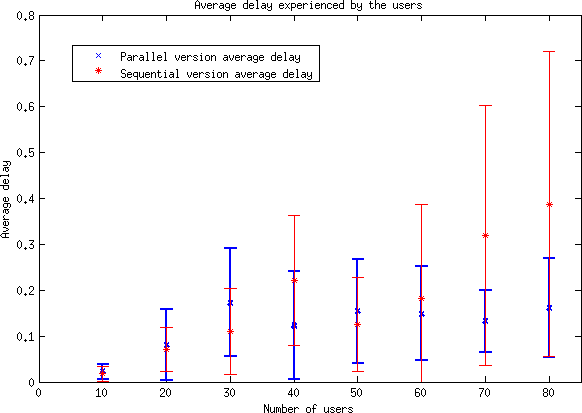
\includegraphics[width=135mm]{plot_users.png}
\caption{Comparison of average message delay with different number of users}
\label{test_1}
\end{figure}


In Fig. \ref{test_2} are presented the results of another experiment. Here the test setup is as follows - there are always 10 clients, each sending a message that has to be received by everyone every half a second. The variable in the test is the total number of messages each sends, which is between 50 and 1000. Since the clients operate completely sequentially and are not particularly efficient, but still have to process all messages from all clients, 1000 was the highest number of messages before I hit the limitation of the test machine.  

I choose this setup in order to evaluate what is the performance penalty of using revisions. Since the number of clients is low, both servers can process all messages before the next burst from all the clients. They do not pile up and the delay is only bound by how quickly each version processes the messages. We can see that sequential version has consistently slightly better average delays and deviation as expected (since the concurrent one has to perform more work per messages, see \ref{imp_no}). We can see that the overhead of the Concurrent revisions is constant and the performance is close to that of the sequential version.
  
\begin{figure}[ht!]
\centering
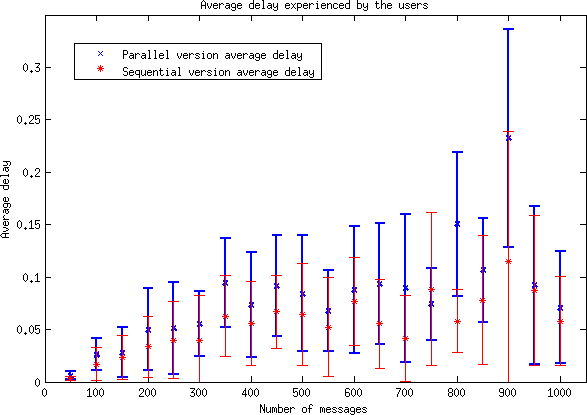
\includegraphics[width=135mm]{plot_m_10.png}
\caption{Comparison of average message delay with different number of messages}
\label{test_2}
\end{figure} 

\section{Future work}
Nowadays systems have increasing capabilities for hardware parallelism. This cannot be explored by the current implementation. A possible future work, based on the concept of Concurrent revisions and the implementation in this project, is to try to incorporate more system threads into the concept. The Lwt library is a cooperative threads library for OCaml\cite{lwt}. It can be used to extend the current implementation with support for actual parallelism and examine the trade-offs of synchronizing system threads with Concurrent revisions.

This could be taken one step further by looking into the possibility of having revisions that are synchronized between distributed nodes. It would be interesting to see what has to be modified in the concept guarantees in order to apply it in a distributed way.

The use case of the chat server could also be used for future work basis. Implementing different chat protocols, such as Extensible Messaging and Presence Protocol (XMPP)\cite{xmpp}. 

Other use cases could also be used to evaluate the concept in the world of OCaml. If these use cases are concerned with problems of different nature to those discussed in the project, they could provide valuable insight on the set of problems suitable for concurrent revisions. Example of these could be games or a file system. These problems require different degree and flavour of determinism and consistency than the server of a centralized system. They could show whether and how Concurrent revisions could be used to implement these guarantees. 

\cleardoublepage
\chapter{Conclusion}

Throughout this project I have designed and implemented a library that incorporates the ideas of Concurrent Revisions and ensured its correctness with a number of unit tests. Together with some small example code, two use cases were produced using the library - a logging system and a chat service. They were used to evaluate the performance and usability of the implementation and the whole concept in the world of OCaml.

We saw that my implementation of Concurrent revisions provides elegant and easy to use interface for introducing concurrency in easy to reason about style. The two use cases confirmed that this concept is indeed applicable for many systems that can benefit from extra concurrency. We also saw that the overhead of a single task done is a revision is acceptable and the improvement that could be gained by concurrency done with revisions is considerable.

There are some remaining issues with this particular implementation. However, they do not belittle the evaluation, findings and conclusion of this project. As a future work these issues could be resolved, which would result in a safer and more elegant implementation.

The findings of this project could be used as a basis for future work. It would be particularly interesting to examine to what extent Concurrent revisions can explore hardware parallelism in OCaml. This could be taken even further by trying to incorporate the ideas of Concurrent revisions in distributed computations.       


\cleardoublepage

%%%%%%%%%%%%%%%%%%%%%%%%%%%%%%%%%%%%%%%%%%%%%%%%%%%%%%%%%%%%%%%%%%%%%
% the bibliography

\addcontentsline{toc}{chapter}{Bibliography}  
\bibliography{refs} 
\cleardoublepage 
\nocite{*}
%%%%%%%%%%%%%%%%%%%%%%%%%%%%%%%%%%%%%%%%%%%%%%%%%%%%%%%%%%%%%%%%%%%%%
% the appendices
\appendix


\chapter{Project Proposal}

%%%%%%%%% Suggested by JMB %%%%%%%%%%%%


\newcommand{\al}{$<$}
\newcommand{\ar}{$>$}

\parindent 0pt
\parskip 6pt

\begin{document}

\thispagestyle{empty}

\rightline{\large{Dimitar Popov}}
\medskip
\rightline{\large{Homerton College}}
\medskip
\rightline{\large{CRSID: DPP23}}

\vfil

\centerline{\large CST Part II Personal Project Proposal}
\vspace{0.4in}
\centerline{\Large\bf Concurrent Revisions Library for OCaml}
\vspace{0.3in}
\centerline{\large {12/10/2013}}

\vfil

{\bf Project Originator:} Dr Anil Madhavapeddy

\vspace{0.1in}

{\bf Resources Required:} See attached Project Resource Form

\vspace{0.5in}

{\bf Project Supervisor:} Dr Anil Madhavapeddy

\vspace{0.2in}

{\bf Signature:}

\vspace{0.5in}

{\bf Director of Studies:} Dr Bogdan Roman

\vspace{0.2in}

{\bf Signature:}

\vspace{0.5in}

{\bf Overseers:} Dr Richard Gibbens and Prof Larry.Paulson

\vspace{0.2in}

{\bf Signatures:} 

\vfil
\eject

\section*{Introduction and Description of the Work}

Concurrency is essential for almost all modern applications. Ensuring good responsiveness and exploiting hardware parallelism is vital but often makes applications difficult to test, maintain and reason about. This usually involves data sharing between different tasks and complicated locking schemes to ensure that the shared data is never corrupted. However  this ofter limits parallelism and could be the root of a number of terrifying and hard to find bugs.

An alternative approach to parallel programming is described in the paper referenced bellow[1]. In this framework the main unit of concurrency are asynchronous tasks called revisions. They are completely isolated using replication and can be forked and joined much like typical asynchronous tasks. The programmer declares what data is shared between revisions using different isolation types. Merge conflicts are resolved deterministically which simplifies the reasoning behind the run-time execution. 

\section*{Resources Required}

The project will be undertaken on my personal laptop (which can be easily replaced in case of failure in less than 5 working days). Naturally the main programming language for the project will be OCaml and will take advantage of the Core and Async libraries for OCaml. Git will be used for source and revision control and Github for backup.

\section*{Starting Point}

As part of my course I have gained a fair understanding of concurrent programming and the main issues it faces. The concept of Concurrent revisions was unfamiliar to me prior to reading the paper, but is simplistic enough to be understood fairly quickly. I have a limited experience with OCaml and some of its core features are new to me. To address this I plan to dedicate the first phase of the project to gaining deeper knowledge of the programming language and what the Core and Async libraries could offer.

\section*{Substance and Structure of the Project}

The aim of the project is implementing an OCaml library for Concurrent revisions. The library must provide the main facilities for parallel programming discussed in the paper - revisions, isolation types, deterministic conflict resolution. An important part of the project should be dedicated to testing the correctness of the behaviour of the library and investigation of its performance. The latter should be done by a number of use cases that would allow comparison with the result obtained by the authors of the paper with their C\# implementation.


The project has the following main sections:

\begin{enumerate}

\item Familiarization with the OCaml programming language and the Core library. Design of the data structures to be used inside the library and the interface that would be exposed to the programmer. Both would most probably be influenced by the original implementation, though given the huge difference between C\# and OCaml, this would not be a trivial task and would require careful consideration in order to produce a clear OCaml version of the concept which is not awkward to use.

\item Developing the implementation of the library. Producing some relatively simple automated tests which would help finding bugs promptly during the development process.

\item Evaluation of the library: Developing a few use cases that would be used to measure the performance of the library. Both a single-threaded and a parallel version (using revisions) should be developed in order to be able to measure memory and CPU overhead. One of these use cases would be a simple char server. Other use cases that explore unpredictable I/O and extensive data sharing should be designed at this stage. Given the limitations of OCaml for exploring hardware parallelism, the versions using Concurrent Revisions are not expected to outperform the sequential versions of the use cases.

\item Optional stage: If time permits, optimization of the library. This stage would became critical if the performance is unsatisfactory.

\item Writing the Dissertation.

\end{enumerate}


\section*{Success Criteria}

The following should be achieved:

\begin{itemize}

\item Implement the library

\item Design the automated tests and pass them

\item Design the use cases for evaluation

\item Measure the performance of the implementation and confirm it is close to the original implementation.

\end{itemize}


\section*{Timetable and Milestones}

\subsection*{Weeks 1 to 3 (28th October - 10th November)}

Familiarize with the OCaml programming language in greater depth (specifically the primitives the language provides for concurrency, the module system and the OOP features of the language.) 

Milestones: Gain good understanding of the mentioned OCaml features as a prerequisite for the further part of the project. 


\subsection*{Weeks 4 to 5 (11th November - 24th November)}

Produce a high level design of the implementation and the interface that will be exposed outside the library. Discussion with supervisor about the suitability of the design and its weak points.

Milestones: Formal design of the library

\subsection*{Week 6 to 9 (25th November - 22nd December)}

Begin implementation of the library. Design automated tests to be used for monitoring the correctness of the implementation.

Milestones: First prototype that should pass the automated tests.

\subsection*{Weeks 10 to 13 (6th January - 9th February)}

Continue the development of the library and implement all of the features, expand the tests if necessary. Attempt trivial optimizations.

Milestones: Second prototype of the library, which potentially, apart of bug fixes and future optimizations, should be deliverable. Progress report submission  

\subsection*{Weeks 14 to 17 (10th February - 9th March)}

Design and implement the use cases required for evaluation. At least two use cases should be produced - both with simple sequential version and one that makes use of the Concurrent Revisions library 

Milestones: Working versions of the use cases.


\subsection*{Weeks 18 to 19 (10th March - 23th March)}

Evaluation and testing. Measure and analyze the performance of the use cases. Determine whether there is need for optimization (discuss with supervisor).

Milestone: Analysis of the performance of the implementation. List of known bugs.


\subsection*{Weeks 20 to 22 (24th March - 13th April)}

Depending on the evaluation and testing results, balance workload between bug fixes and optimization of the project and exam preparation

Milestones: Confirm any known bugs are fixed and performance is satisfactory.


\subsection*{Weeks 23 to 26 (14th April - 11th May}

At this stage the work on the project should hopefully be complete. Write the Dissertation and do one final review of the whole project.

Milestones: Submit Dissertation



\section*{Reference}
\begin{description}
\item{[1]} \emph{Concurrent Programming with Revisions and Isolation Types}, Sebastian Burckhardt, Alexandro Baldassion, and Daan Leijen. OOPSLA'10

\end{description}

\newpage

\section*{Project Resource Form}
No special resources are required. I plan on using my personal laptop (dual-core i5, 4GB RAM). In case of hardware failure I have a spare machine with similar specification. I accept full responsibility for this machine and I have made contingency plans to protect myself against hardware and/or software failure.

For source control I am going to use Git and for backup - Github.

I plan on using the Core and Async libraries for OCaml extensively, both of which are publicly available.


\end{document}



\end{document}
